% COMPILE WITH LuaLatex !!!

% Other paper formats are possible: aspectratio = 43 (4:3), 169 (16:9)
%\documentclass[aspectratio=43,handout]{beamer}
\documentclass[8pt, t,
aspectratio=169,% for widescreen (16:9) presentations
%aspectratio=43,% for traditional (4:3) presentations
%handout,% UNCOMMENT to deactivate slide animation (overlays)
]{beamer}

\usepackage[utf8]{}
\usepackage[T1]{fontenc}

% Title and author
\title{Beamer\\Template} % If needed, manually add line breaks with "\\"
\author[Dr. sc. Sebastian Schwindt]{Dr. sc. Sebastian Schwindt}
\subtitle{Example}

\usetheme{lww}


\begin{document}

% Create the titlepage
\maketitle

% Optional: show the outline
\begin{frame}{Outline}
	\tableofcontents
\end{frame}

%%%%%%%%%%%%%%%%%%%%%%%%%%%%%%%%%%% slides %%%%%%%%%%%%%%%%%%%%%%%%%%%%%%%%%%%%%
\section{Navier-Stokes Equations}
\subsection{an example}

\begin{frame}{\secname: \subsecname}
	\bigskip
	\fcolorbox{orange_med}{orange_light}% find more colors in the style file
	{%
		\parbox{\textwidth}{The Navier-Stokes equations mathematically express \textbf{momentum} and \textbf{mass continuity} for \textbf{Newtonsche fluids}.}%
	}\bigskip
	
	
	\subsection{Mass and Momentum Conservation}
	\textbf{Mass conservation} 
	\begin{equation*}
	 	\frac{\partial \rho}{\partial t} + \frac{\partial \rho u_x}{\partial x}  + \frac{\partial \rho u_y}{\partial y} + \frac{\partial \rho u_z}{\partial z} = 0
	\end{equation*}
	
	\textbf{Momentum conservation}
	\begin{align*}
		\textcolor{orange_med}{\rho g_x} \textcolor{green_med}{- \frac{\partial p}{\partial x}} + \textcolor{blue_med}{\mu \left(\frac{\partial^2 u_x}{\partial x^2}  + \frac{\partial^2 u_x}{\partial y^2} + \frac{\partial^2 u_x}{\partial z^2}\right)} & = \rho \left(\textcolor{red!90}{\frac{\partial u_x}{\partial t}} + \textcolor{blue!90}{u_x\frac{\partial u_x}{\partial x} + u_y\frac{\partial u_x}{\partial y} + u_z\frac{\partial u_x}{\partial z}}\right)\\	 	
		\textcolor{orange_med}{\rho g_y} \textcolor{green_med}{- \frac{\partial p}{\partial y}} + \textcolor{blue_med}{\mu \left(\frac{\partial^2 u_y}{\partial x^2}  + \frac{\partial^2 u_y}{\partial y^2} + \frac{\partial^2 u_y}{\partial z^2}\right)} & = \rho \left(\textcolor{red!90}{\frac{\partial u_y}{\partial t}} + \textcolor{blue!90}{u_x\frac{\partial u_y}{\partial x} + u_y\frac{\partial u_y}{\partial y} + u_z\frac{\partial u_y}{\partial z}}\right)\\	 	
		\textcolor{orange_med}{\rho g_z} \textcolor{green_med}{- \frac{\partial p}{\partial z}} + \textcolor{blue_med}{\mu \left(\frac{\partial^2 u_z}{\partial x^2}  + \frac{\partial^2 u_z}{\partial y^2} + \frac{\partial^2 u_z}{\partial z^2}\right)} &= \rho \left(\textcolor{red!90}{\frac{\partial u_z}{\partial t}} + \textcolor{blue!90}{u_x\frac{\partial u_z}{\partial x} + u_y\frac{\partial u_z}{\partial y} + u_z\frac{\partial u_z}{\partial z}}\right)
	\end{align*}
\end{frame}

\section{Images}
\subsection{an example}
\begin{frame}{\secname: \subsecname}
	\begin{columns}[c]
		\begin{column}{.8\textwidth}
			\sscFig{salome-hydro}{A figure caption}
		\end{column}
	\end{columns}
\end{frame}

\section{Videos}
\subsection{an example}
\begin{frame}{\secname}
	\textbf{\subsecname}\\\medskip
	\centering
	\movie[externalviewer]{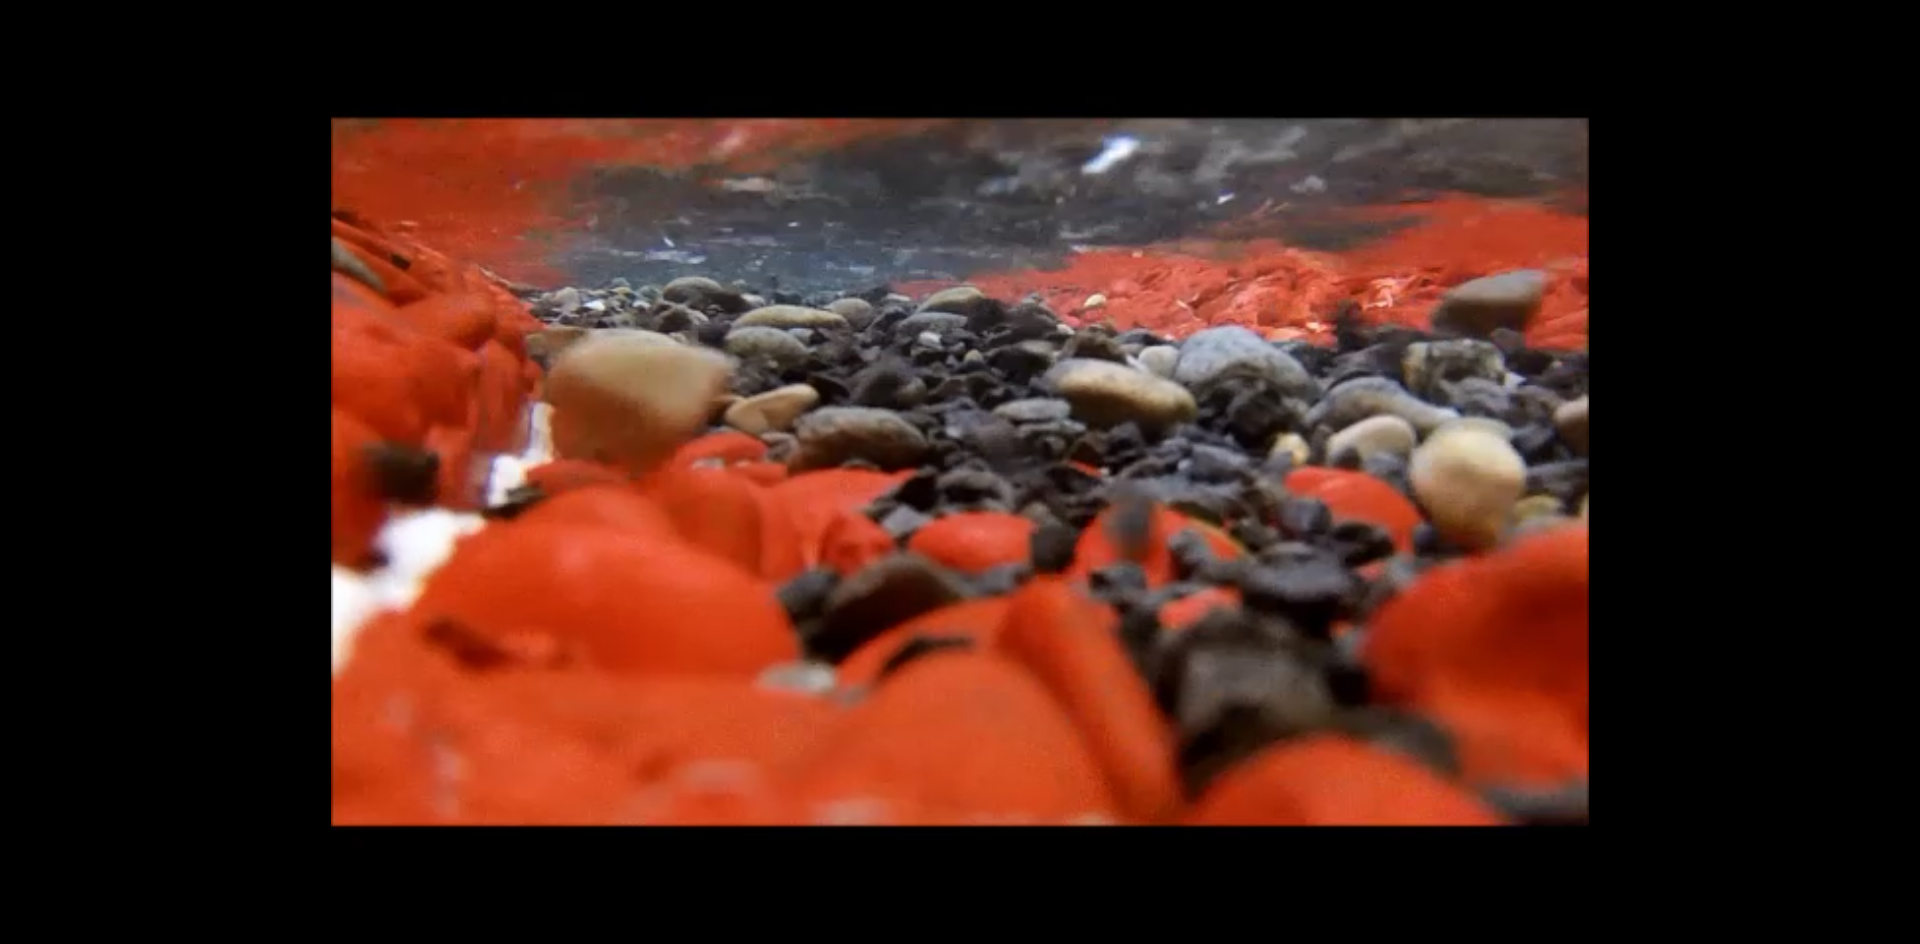
\includegraphics[width=0.78\textwidth,keepaspectratio]{videos/thumbnail-bedload-example.jpg}}{videos/bedload-example.mp4}\\
	\begin{center}
		\textit{An example video with thumbnail (source: \sscURL{Schwindt 2015}{https://infoscience.epfl.ch/record/229862/files/EPFL\_TH7655.pdf})}
	\end{center}
\end{frame}

\section{Code and Color Blocks}
\subsection{fragile frames}
\begin{frame}[fragile]{\secname: \subsecname}
	An example FRAGILE frame with code blocks - attention: $[fragile]$ is needed for code blocks
	\begin{columns}[T]
		\begin{column}{.48\textwidth}
			\begin{lstlisting}[numbers=none]
				git status
				[optional] git diff
				git add .
				git commit -m "Modified ..."
				git pull --rebase
				git push
			\end{lstlisting}
		\end{column}
		\begin{column}{0.48\textwidth}
			\vspace{-0.18cm}
			\begin{tcolorbox}[colback=green_warm, colframe=orange!20!white, bottom=0mm, middle=0mm, boxsep=0.2mm, opacityframe=0.8, opacityfill=0.2, size=fbox]
				$\rightarrow$ verify files that you modified\vspace{0.09cm}\\\vspace{0.09cm}
				$\rightarrow$ see what exactly changed (optional)\\\vspace{0.09cm}
				$\rightarrow$ stage changed files $\rightsquigarrow$ DOT adds all	\\	\vspace{0.09cm}	
				$\rightarrow$ commit changes and provide a message \\\vspace{0.09cm}
				$\rightarrow$ verify integrity of local and remote changes\\\vspace{0.09cm}
				$\rightarrow$ push changes\vspace{0.2cm}
			\end{tcolorbox}
		\end{column}
	\end{columns}
	\begin{tcolorbox}[colbacktitle=gray!45!white, colback=gray!25!white, fonttitle=\bfseries, standard jigsaw,colframe=gray!25!white, bottom=0mm, middle=0mm, boxsep=0.2mm, opacityframe=0.5, opacityfill=0.7, opacitybacktitle=0.95, title filled, title=Inline code blocks, size=fbox]	
		\textcolor{green_warm}{	
			Use a colorbox \colorbox{black!80!blue}{\lstinline{to display code}} or no colorbox \lstinline{to display code}
		}
	\end{tcolorbox}
\end{frame}

\section{Working with TIKZ}
\begin{frame}{\secname}
	\textbf{An example for creating a tikzpicture}
	\begin{itemize}
		\item more predefined shapes can be read from the beamerlww.sty style file
	\end{itemize}\bigskip
	\begin{columns}[c]
		\begin{column}{.5\textwidth}
			\begin{tikzpicture}
				\draw[dashed,color=red!60] (0,0) arc (-90:90:0.5 and 1.5);% right half of the left ellipse
				\draw[semithick] (0,0) -- (4,1);% bottom line
				\draw[semithick] (0,3) -- (4,2);% top line
				\draw[semithick,color=red!90] (0,0) arc (270:90:0.5 and 1.5);% left half of the left ellipse
				\draw[semithick,color=blue!90] (4,1.5) ellipse (0.166 and 0.5);% right ellipse
				% inflow pars
				\draw (-0.45,2.4) node {\textcolor{red!90}{Area $A_1$}};
				\draw (-0.1,1.5) node {\textcolor{red!90}{$u_1 \mathbf{\leadsto}$}};
				\draw (0,-0.3) node {\textcolor{red!90}{$Q_{1} = u_1\cdot A_1$}};
				% outflow pars
				\draw (3.8,2.4) node {\textcolor{blue!90}{Area $A_2$}};
				\draw (4.35,1.5) node {\textcolor{blue!90}{$\mathbf{\leadsto} u_2$}};
				\draw (4.0,-0.3) node {\textcolor{blue!90}{$Q_{2} = u_2\cdot A_2$}};
			\end{tikzpicture}
		\end{column}
	\end{columns}
\end{frame}

\section{Animations}
\begin{frame}{\secname}
	\textbf{Another TIKZ picture that appears only on click}\bigskip
	\onslide<2->{
	\begin{columns}[c]
		\begin{column}{0.3\textwidth}
			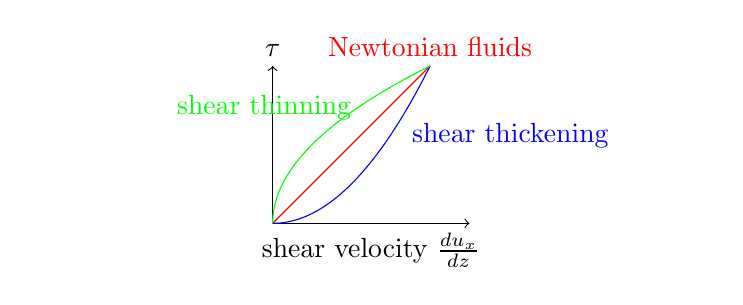
\begin{tikzpicture}[domain=0:4]
				\draw[->] (-0.,0) -- (2.5,0) node[pos=0.5,below] {\parbox{0.7\textwidth}{\centering shear velocity $\frac{d u_x}{d z}$}};
				\draw[->] (0,-0.) -- (0,2) node[above] {$\tau$};
				\draw[scale=1.0, domain=0:2, smooth, variable=\x, red] plot ({\x}, {\x}) node[above] {Newtonian fluids};
				\draw[scale=1.0, domain=0:2, smooth, variable=\d, blue] plot ({\d}, {\d * \d * 0.5}) node[yshift=-25,xshift=-10,right] {shear thickening};
				\draw[scale=1.0, domain=0:1.414, smooth, variable=\s, green] plot ({\s*\s}, {\s*1.414}) node[yshift=-15,xshift=-25,left] {shear thinning};
			\end{tikzpicture}
		\end{column}
	\end{columns}
	}
\end{frame}



%%%%%%%%%%%%%%%%%%%%%%%%%%%%%%%%% final slide %%%%%%%%%%%%%%%%%%%%%%%%%%%%%%%%%%
% Two options: white and blue bg
\thankyou{Thank you for listening}{Dr. sc. (PhD) Sebastian Schwindt}{sebastian.schwindt@iws.uni-stuttgart.de}{+49 (0)711 phone}{theme/logos/drop.png}
% \thankyoublue{Thank you}{Dr. sc. Sebastian Schwindt}{sebastian.schwindt@iws.uni-stuttgart.de}{+49 (0)711 685 64 789}{theme/logos/drop.png}
	
\end{document}
